% ToDo: General text about the method...
In this chapter the the methodology that was used to facilitate the making of this master thesis is describe. 
Finding appropriate feature candidates was one of the first challenges faced in this work. There are a significant amount of papers discussing potential candidates to bring in to the model, those with similar conditions has inspired the selection of features and they are reviews in chapter \ref{ss:literature_review}. When the selection of features was completed a search for appropriate data sources begun. All the required information was found from open data source. To facilitate the data capture and transformation a toolbox of shell- and Python scripts was created. Generation of the feature space was performed by a Scala application that rendered the features to the database and for future processing by Weka. In this stage the features were normalised and abnormal records where dismissed. For a detailed description of this process see chapter \ref{sss:data_cleansing}. The built in PCA and MLP functionality of Weka was used to select the features that contributed most to the solution of the model. Weka was enriched with a hyperbolic tangent activation function to promote the ability to capture the non-linearities in the model, see chapter \ref{sss:weka_tanh} for further details. Early testing indicated that hyperbolic tangent outperformed the traditional sigmoid activation function, both with respect to the performance of the model and the speed of convergence of the gradient decent algorithm. Finally the selected features was exported to Weka's native file format ``arff''.
\\
Comparison with a more traditional machine learning algorithm is one of the major prerequisites of this paper. To stage this a commonly used Python library named LibSVM was used. A Python script reads the Weka data file (arff), partitions it into three parts, builds the model and validates it. Tuning of the SVR was done by iterating over a separate interval for each parameter searching for the appropriate values by evaluating the model against the test data set. As the icing on the cake some additional traits are added to the multilayer perceptron calculations like: conformal predictions, random initialization of weights, adjustable learning rates and momentum. Finally the parameters for the MLP algorithm is fine tuned and the definitive result is presented in chapter \ref{ss:results}.  
\\

The main features of the work flow is as follows: 
\begin{itemize}
\item Identify potentially useful features to include in model
\item Find data sources for features
\item Capture data from selected sources
\item Generate feature space
\item Perform principal components analyse (PCA) on features 
\item Select features for model
\item Compare performance between multilayer perceptron (MLP) and support vector regression (SVR)
\item Incorporate additional functionality to multilayer perceptron
\item Fine tune multilayer perceptron parameters
\item Evaluate result
\end{itemize}

%========================================
%===
%=== Data collection
%===
%========================================
\subsection{Data collection}
All data sources used in this research are publicly available, so called ``Open Data''. The Swedish parliament has issued a directive that requires all government departments and municipality's to make there data publicly available. This is one of the major reasons behind the rich variety of information available from the municipality of Stockholm witch is one of the major information sources.  
\\
The information gathering is done incremental starting with the retrieval of a list containing the streets of central Stockholm from the website svenskagator.se \cite{dat}{Sven:13}. This list is read into the MySQL database handling the persistent data, see chapter \ref{sss:street_load}. The list of streets are then used to fetch the final prices of sold apartments for the given time period, one a per street basis from slutpris.se \cite{dat}{Slut:13}. For details see chapter \ref{sss:slutpris}.

%***
%* Streets searched for sales
%***
\subsubsection{Streets searched for sales} \label{sss:street_load}
Street names from svenskagator.se \cite{dat}{Sven:13} is read from the site using the unix command line tool curl and processed by a born shell script that produces a SQL file witch contains insertion statements. This file is then used to load the MySQL database with the street names. In total 1341 street names is read into the database.
\\

%***
%* Apartment sale statistic
%***
\subsubsection{Apartment sale statistic} \label{sss:slutpris} %from slutpris.se
Information from the REST API at slutpris.se \cite{dat}{Slut:13} is structured according to the Json standard. A program written in Scala is used to retrieve the information from slutpris.se. For each street in the list specified in chapter \ref{sss:street_load} a separate HTTP request has to be performed, the response is retrieved, parsed and transformed into class instances that are stored in the database. The request URL and parameters for the REST call is as specified in table \ref{tab:slutpris_se}. Features collected from slutpris.se is described in table \ref{tab:slutpris_se_result}. 

\begin{table}[H]
\centering
\begin{tabular}{ |p{2cm}|p{2cm}|p{2cm}|p{2cm}| } 
\hline
\multicolumn{4}{|c|}{http://slutpris.se/main\_application/get\_search\_result/} \\
\hline
dateLimit & order & minrum & maxrum \\
minarea & maxarea & minpris & maxpris \\
minavg & maxavg & area &  \\
\hline
\end{tabular}
\caption{Request to slutpris.se}
\label{tab:slutpris_se}
\end{table}


\begin{table}[H]
%\centering
\begin{tabular}{ | p{5.6cm} | p{5.6cm} | } 
\hline 
\multicolumn{2}{|c|}{Feature} \\
\hline
Construction year of building & Building has elevator \\
Fireplace in apartment & Apartment has a duplex \\
Apartment is a penthouse & Apartment has balcony \\
Date of transaction & Price per square meter \\
Area in square meters & Number of rooms, kitchen excluded \\
Stores from the street level & Monthly fee payed to association \\
Selling price & Latitude and longitude coordinates \\
Street address of apartment & Name of reltor \\
Reltor identification &  \\
\hline
\end{tabular}
\caption{Attributes in response from slutpris.se}
\label{tab:slutpris_se_result}
\end{table}

Apartment statistics are gathered for transactions finalized in the time frame 2011-08-01 until 2013-06-08. In total about 8900 transactions are fetched from slutpris.se, they are then filtered and only apartments in the bounding box defined in table \ref{tab:sthlm_bounding_geobox}. For more information regarding the generation and cleaning of the data se chapter \ref{sss:data_cleansing} and \ref{sss:feature_aggregation} respectively.

\begin{table}[H]
%\centering
\begin{tabular}{ | l | l | l | } 
\hline 
Type & Min & Max \\
\hline
Latitude & 59.298149 & 59.356296 \\
Longitude & 18.021784 & 18.115082 \\
\hline
\end{tabular}
\caption{Bounding box of centre of Stockholm}
\label{tab:sthlm_bounding_geobox}
\end{table}


%***
%* Street information
%***
\subsubsection{Street information} \label{sss:street_info}
Information retrieved from slutpris.se is enhanced with the zip code and latitude and longitude are replaced with more accurate information retrieved from the open data portal of Stockholm's municipal, openstreetws.stockholm.se \cite{dat}{smos:13}. Sales statistics are sparse compared to the number of unique street addresses in the surveyed area. Those a lazy evaluating solution is more efficient then pre loading all the adequate data prior to the substitution. The solution is based on a caching schema that uses the database to persist the retrieved information. When a street address is searched a lookup in the cache is done, if the information is available in the cache it is returned to the requester. If the street address is not in the cache it is retrieved from Stockholm's open data portal.  Enhancement of the sales statistic is achieved by looping throw all entry's of the sales statistic and for each entry lookup the street information from the cache. 

%***
%* Historic inflation figures
%***
\subsubsection{Historic inflation figures} \label{sss:hist_inflation}
Statistics over the apartments sales is derived from a two year period and therefore inflation has an impact on the sales price over time, closed sales from 2011 would appear to have a actual lower price then more resent deals. To avoid this bias on the price feature the final sales price is adjusted according to the monthly inflation up to the last date of the examined time interval. Inflation statistics was retrieved from the Statistics Sweden (SCB) who is responsible for the official inflation figures. Information regarding the inflation rate \cite{dat}{Scb2:13} and underlying inflation rate \cite{dat}{Scb1:13}. The retrieved information is pre processed by a Python script and then read into the database.  

%***
%* Interest rates for apartment loans
%***
\subsubsection{Interest rates for apartment loans} \label{sss:interest_rates}
There is a ongoing debate regarding the interest rates influence on the sales price of apartments in Stockholm. The prerequisite for being able to examine whether the interest rate has an impact on the sales price, historical interest rates were fetched from Skandinaviska Enskilda Banken (SEB) \cite{dat}{SEB:13} and Swebank \cite{dat}{Sweb:13}. This information was temporary stored as CSV-files, pre processed by a Python script and inserted into the database. 

%***
%* National election result
%***
\subsubsection{National election result} \label{sss:election_stats}
Political preferences of buyers, neighbours and policies of governing parties is a potential feature that affects the market. Statistics from the previous Swedish election in 2010 and geographic information of the layout of the constituency's are available from the Swedish authority Valmyndigheten \cite{dat}{Valm:13}. This statistics were downloaded as Excel files and loaded into the database via a Python script. Geographic information regarding the constituency's layout is supplied as so called shape files. The coordinates is transformed and the GeoTool Java library is used to find out witch constituency a given apartment belongs to and its unique id. Finally this id is used to find the election figures from the database.

%***
%* Local features
%***
\subsubsection{Local features} \label{sss:local_features}
Stockholm's municipal \cite{dat}{sthlm:13} provides data about over eighty local feature types. Fourteen of those were selected as candidates for the models feature space. Each feature has a unique identifier that has to be fetched from a catalogue using REST-calls. This catalogue was retrieved whit the unix tool curl and stored in XML-format, a Python script reads the file en inserts the unit types into the database. A second Python script reads the entries of the selected feature types from the REST-service and stores them into the database. Each feature entry is associated with a geographic coordinate (latitude and longitude), this information is used when the feature space is generated to calculate the distance to the nearest feature of each type.   

\begin{table}[H]
%\centering
\begin{tabular}{ | l | l | } 
\hline 
\multicolumn{2}{|l|}{http\://api.stockholm.se} \\
\hline
\hline
Type & URL \\
\hline
unit types & /ServiceGuideService/ServiceUnitTypes \\
unit entry & /ServiceGuideService/ServiceUnitTypes/\{id\}/ServiceUnits \\
\hline
\end{tabular}
\caption{REST services at api.stochlolm.se}
\label{tab:feature_rest}
\end{table}


%========================================
%===
%=== Features
%===
%========================================
\subsection{Features} \label{sss:features}
The features can be classified into six major groups depending on there data domain and origin. The groups are in order taken from table 
\ref{tab:feature_list1}: sales information regarding the apartment, geographical reference information, distance to local feature units and from table
\ref{tab:feature_list2}: geographic position, interest rates, election result from 2010. A complete listing of all the features used to create the model can be found in appendix \ref{sss:appendix_a}.

%***
%* 
%***
\subsubsection{Feature aggregation} \label{sss:feature_aggregation}
At the point in time when the generation of the feature space occurs all the required data has been loaded into the database.
\\
\texttt{ToDo: More stuff...}

%\subsubsection{Description of Features} \label{sss:feature_description}
%\begin{table}[H]
%\centering
\begin{tabular}{ | l | l | p{7cm} | } 
\hline 
Nr & Feature & Description \\
\hline
\hline
1 & construction\_year & Year when the building was constructed \\
2 & elevator & Building has elevator installed \\
3 & fireplace & Fireplace available in apartment \\
4 & duplex & Apartment has a duplex \\
5 & penthouse & Apartment is a penthouse \\
6 & balcony & Apartment has balcony \\
7 & squares & Area of apartment in square meters \\
8 & rooms & Total number of rooms, kitchen excluded \\
9 & floor & Apartments floor, numbers of stores from the street level \\
10 & fee & Anual fee payed to the housing association \\
11 & agencyid & Reltor identification \\
\hline
12 & postal\_code & Zip code \\
13 & fix\_point\_1 & Distance in meters to KTH Royal Institute of Technology \\
14 & fix\_point\_2 & Distance in meters to The Royal Palace of Stockholm \\
15 & fix\_point\_3 & Distance in meters to Sergels Torg (CBD) \\
\hline
16 & jog\_track\_dist & Distance in meters to nearest jogging track \\
17 & pad\_pool\_dist & Distance in meters to nearest wading pool \\
18 & daycare\_dist & Distance in meters to nearest daycare center \\
19 & pool\_dist & Distance in meters to nearest pool facility \\
20 & open\_daycare\_dist & Distance in meters to nearest daycare center \\
21 & sports\_hall\_dist & Distance in meters to nearest sports hall \\
22 & outdoor\_gym\_dist & Distance in meters to nearest out door gymnasium \\
23 & sports\_field\_dist & Distance in meters to nearest sports field\\
24 & playing\_field\_dist & Distance in meters to nearest palying field \\
25 & library\_dist & Distance in meters to nearest common library\\
26 & env\_station\_dist & Distance in meters to nearest environment station \\
27 & preschool\_dist & Distance in meters to nearest preschool \\
28 & bath\_dist & Distance in meters to nearest bath facility \\
29 & playground\_dist & Distance in meters to nearest play ground \\
30 & subway\_dist & Distance in meters to nearest subway station \\
31 & station\_dist & Distance in meters to nearest train or commuter train station. \\
32 & park\_dist & Distance in meters to nearest park \\
33 & forest\_dist & Distance in meters to nearest forest \\
34 & water\_dist & Distance in meters to nearest watercourse \\
\hline
\end{tabular}
\caption{List of features part 1}
\label{tab:feature_list1}
\end{table}

\begin{table}[H]
%\centering
\begin{tabular}{ | l | l | p{7cm} | } 
\hline 
Nr & Feature & Description \\
\hline
\hline
35 & lat & Latitude given as decimal number coded in WGS84 \\
36 & lng & Longitude given as decimal number coded in WGS84 \\
37 & zone1 & Id of grid square where apartment is located, taken from a 7x7 grid. \\
38 & zone2 & Id of grid square where apartment is located, taken from a 9x9 grid. \\
\hline
39 & seb\_interest\_3m & SEB's interest rate for a 3 month bound loan when the apartment was sold \\
40 & seb\_interest\_2y & SEB's interest rate for a 2 year bound loan when the apartment was sold \\
41 & seb\_interest\_5y & SEB's interest rate for a 5 year bound loan when the apartment was sold \\
42 & seb\_interest\_10y & SEB's interest rate for a 10 year bound loan when the apartment was sold \\
43 & swebank\_interest\_3m & Swebank's  interest rate for a 3 month bound loan when the apartment was sold\\
44 & swebank\_interest\_2y & Swebank's interest rate for a 2 year bound loan when the apartment was sold \\
45 & swebank\_interest\_5y & Swebank's interest rate for a 5 year bound loan when the apartment was sold \\
46 & swebank\_interest\_10y & Swebank's interest rate for a 10 year bound loan when the apartment was sold \\
\hline
47 & proc\_M & Proportion of votes in local constituency won by Moderata samlings\-partiet \\
48 & proc\_C & Proportion of votes in local constituency won by Centerpartiet \\
49 & proc\_FP & Proportion of votes in local constituency won by Folkpartiet Liberalerna \\
50 & proc\_KD & Proportion of votes in local constituency won by Kristdemokraterna \\
51 & proc\_S & Proportion of votes in local constituency won by Sveriges social\-demo\-kratiska arbetare\-parti \\
52 & proc\_V & Proportion of votes in local constituency won by V{\"a}nsterpartiet \\
53 & proc\_MP & Proportion of votes in local constituency won by Milj{\H o}partiet de Gr{\H o}na \\
54 & proc\_SD & Proportion of votes in local constituency won by Sverige\-demokraterna \\
55 & proc\_Alians & Majority for the Alliance parties \\
56 & proc\_RodGron & Majority for the opposition parties \\
57 & majority\_Alians & Proportion of votes to the majority \\
\hline
\end{tabular}
\caption{List of features part 2}
\label{tab:feature_list2}
\end{table}


%***
%* 
%***
\subsubsection{Cleansing data} \label{sss:data_cleansing}
\texttt{ToDo: More stuff...}

%***
%* 
%***
\subsubsection{Partitioning data} \label{sss:data_partitioning}
The data set was finally partitioned into three distinct datasets used for: training, validation and testing. Prior to the partitioning the rows in the data set it was scrambled (randomly rearranged) to avoid uneven distribution of similar data and thereby distorting the result. After studying the literature referenced in this thesis and observing commonly used data petitioning schemas, a 70\%/15\%/15\% split ratio was selected. On our complete data set with 5991 entries that resulted in the following partitioning.
\begin{table}[H]
\begin{tabular}{ | l | l | l | }
\hline
Partition & Relative size & Number of entries \\
\hline
\hline
Training set & 70\% & 4195 \\
Validation set & 15\% & 898 \\
Test set & 15\% & 898 \\
\hline
\end{tabular}
\caption{Final partitioning of data}
\label{tab:data_partitioning}
\end{table}  

%\subsection{Program construction}
%\subsubsection{Information retrieval and feature construction}
\subsubsection{Enrichment of Weka with hyperbolic tangent activation function} \label{sss:weka_tanh}
%\subsubsection{Analysis tools for PCA and SVR}
%\subsubsection{Modifications to Weka}

%\subsection{Test design}


%========================================
%===
%=== Construction of the Multilayer Perceptron
%===
%========================================
\subsection{Construction of the Multilayer Perceptron} \label{sss:construction_mlp}
Multilayer Perceptrons are a powerful tool used to build predictive models from a set of input data containing a given number of features and as result predict one or more target variables. The topology of a MLP is simple and straight forward, see figure \ref{NeuralNet_InHidHidOut_full}. The network is divided into layers which comes in three flavours: input layer, hidden layers and output layers. For each feature in the input data a separate node is created in the input layer. This layer is followed by one or several so called hidden layers that can contain different number of nodes each and finally a output layer with one or more nodes. In this paper a single output node is used to produce the estimation of the apartment price (regression). When the MLP model is used for classification a so called `Soft Max' is created which consists of one node for each expected class. 
\
\begin{figure}[ht] 
\begin{center}
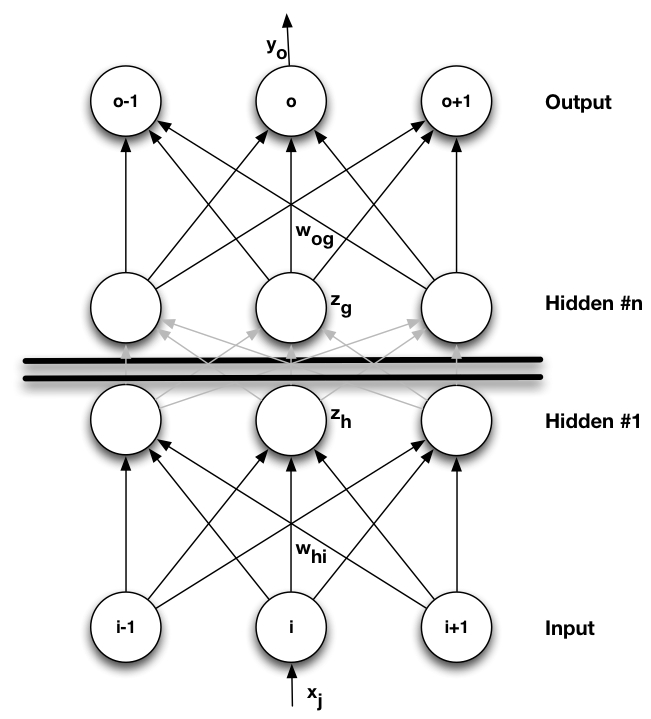
\includegraphics{NeuralNet_InHidOut-full.jpg}
\caption{Layout of \textit{Multilayer Perceptron}.}
\label{NeuralNet_InHidHidOut_full}
\end{center}
\end{figure}

Each nod in the lower layer is connected to all nodes in the layer above and a weight is associated with the connection, for example $w_{hi}$ in figure \ref{NeuralNet_InHidHidOut_full}. The output of a node in the network is calculated with a so called activation function which input is the weighted sum of the incoming connections. Activation functions are covered in subsection \ref{sss:activation_function}. A error function is used to calculate the difference between the output from the network and the target (desire) value, this is typically the mean square error function $E = \frac{1}{2} (t - y)^{2} $ but other functions are also used. In this paper the supervised training algorithm called back-propagation is used to create the statistical model. This algorithm can briefly be described as follows:
\
\begin{enumerate}
\item Sample from the training set is presented (indata to input nodes).
\item Inputs are propagated forward in the network by calculating output values for the nodes in each layer by applying the activation function from input nodes towards output node. \textit{Forward propagation}
\item Output error is calculated by the error function $ E = \frac{1}{2} (t - y)^{2} $. Here $t$ is the target value and $y$ is the output of the network. 
\item \textit{Backward propagation}
\item Calculate the gradient, momentum ($ M(t) = M(t-1) * \lambda - \textit{gradient}$) and update weights ($ W(t) = \alpha * M(t)$), here $\lambda$ = velocity decay, $\alpha$ = learning rate.
\end{enumerate} 
The algorithm described above is applied on the whole testdata set and repeated for the desired number of iterations. At this point all weights are adjusted to represent a god model of the problem. Initialization of the weights are discussed in subsection \ref{sss:weight_bias_initialization}. 
\
Three different regimes of weight updates are often used:
\begin{itemize}
\item \textit{Online}. Weights are updated after every sample in the test dataset. 
\item \textit{Batch}. Weights are updated after passing all training data.
\item \textit{Mini-batch}. Divide the training data set into chunks of equal size and update the weights after passing a chunk.
\end{itemize} 
The selected regime of weight update foremost affects the speed of the learning. In subsection \ref{sss:boosting_mlp_minibatch} the speed gain of using the mini-batch versus batch regime is explored. In some situations the learning algorithm can give rise to so called overfitting which leads to less favourable predictions for the verification set. Overfitting can be avoided by adding noise to the weights, this is future elaborated in subsection \ref{sss:dropout_regime}.
\
The first assessment was to use Weka as the major platform for testing and building models. However it was soon clear that the performance of the platform was to poor to offer a workable environment. Though Weka was used to get a feel of the dataset, test out MLP configurations and perform a principal component analyse. Several MLP configurations were tested and evaluated to gather basic data. The sigmoid activation function was not able to create good models so Weka was supplemented with a hyperbolic tangent function, which outperformed the sigmoid networks and produced good models.  

%***
%* Activation function
%***
\subsubsection{Activation function} \label{sss:activation_function}
\texttt{ToDo: More stuff...}

%***
%* 
%***
%\subsubsection{Cost function}

%***
%* Weight and bias initialization
%***
\subsubsection{Weight and bias initialization} \label{sss:weight_bias_initialization}

\begin{equation} \label{eq:weight_init_regular}
W_{ij} \sim U[-\frac{1}{\sqrt{n_{i-1}}},\frac{1}{\sqrt{n_{i-1}}}]
\end{equation}

normalized initialization
\begin{equation} \label{eq:weight_init_normalized}
W_{ij} \sim U[-\frac{\sqrt{6}}{\sqrt{n_{i-1}+n_{i}}},\frac{\sqrt{6}}{\sqrt{n_{i-1}+n_{i}}}]
\end{equation}

where U[-x,x] is the uniform distribution in the interval $-x < a < x$ and $n_{i}$ is the number of nodes in layer i.

%***
%* Weight update regime
%***
\subsubsection{Weight update regime} \label{sss:weight_regime}
Multilayer perceptron models can with advantage be built with use of the Backpropagation algorithm and have Gradient Descent as one of its corner stones. Choosing a good regime of weight updating is there for crucial. It is more rewarding to follow small but consistent gradients when updating the weights then bigger and more inconsistent ones. In this paper we use two mechanisms to refine the process of updating the weight: learning rate and momentum. 
The concept of adding learning rate can be viewed as a way to control how fast the weights should be learned in a update. For data sets with redundant data the learning rate can be low thou to low learning rate will slow down the learning considerable, to high rate can make the learning overshoot. It is often favourable to keep the learning rate high in the beginning and turning it down further along in the update process.   
\\
The method of using momentum steams from the idea of adding a momentum to the current gradient in the gradient decent algorithm rather then follow the steepest decent. Adding a momentum based on the previous weight updates to the current gradient makes it keep going in the previous direction, a momentum, see equation \ref{eq:wupdate_first}. 

\begin{equation} \label{eq:wupdate_first}
 \mathbf{v}_{t} = \alpha \mathbf{v}_{t-1} - \epsilon \frac{\partial{E_{t}}}{\partial{\mathbf{w}_{t}}} 
\end{equation}

\begin{equation} \label{eq:wupdate_eq}
\Delta \mathbf{w}_{t} = \mathbf{v}_{t} 
\end{equation}

\begin{equation} \label{eq:wupdate_final}
\Delta \mathbf{w}_{t} = \alpha \Delta \mathbf{w}_{t-1} - \epsilon \frac{\partial{E_{t}}}{\partial{\mathbf{w}_{t}}} 
\end{equation}
Weight update can be expressed in terms of the velocity, see equation \ref{eq:wupdate_eq}. Expressing the update in terms of previous weight update gives the equation \ref{eq:wupdate_final}. This combined with the learning rate gives the final update function $\lambda \Delta \mathbf{w}_{t}$ where $\lambda$ is the learning rate and $\alpha$ the momentum multiplier.


%***
%* Dropout regime
%***
\subsubsection{Dropout regime} \label{sss:dropout_regime}
\texttt{ToDo: More stuff...}


%========================================
%===
%=== Optimization with Genetic Algorithm 
%===
%========================================
\subsection{Optimization with Genetic Algorithm}
\texttt{ToDo: More stuff...}

%***
%* Genome
%***
\subsubsection{Genome}
\texttt{ToDo: More stuff...}

%***
%* Objective function
%***
\subsubsection{Objective function}
\texttt{ToDo: More stuff...}

%***
%* Crossover and mutation
%***
\subsubsection{Crossover and mutation}
\texttt{ToDo: More stuff...}

%***
%* The search process
%***
\subsubsection{The search process}
\texttt{ToDo: More stuff...}


